% !TEX root = ../Ausarbeitung.tex
\section{Learned Approaches}
The next approach was trying to learn some of the movements instead of hard-coding them.
We used an evolutionary approach to learn weights for a spiking neural network which controls the robots movements.

\subsection{Evolutionary Approach}
In this approach the robot is controlled by a spiking neural network which can be seen in \autoref{fig:network}.
The network has three input and seven output neurons which are fully connected.
The three dimensional position of the cylinder is used for the input neurons.
Six of the output neurons control the six joints of the robots arm and the last neuron controls when the hand should release the cylinder.

The individuals of our evolutionary algorithm are lists of 21 values each representing one weight of the network.
To evaluate the individuals a throw is simulated and the distance of the cylinder from the table represents the fitness of the individual.
After each individual of a generation is evaluated we select the elite which consists of the best 50\% of the individuals.
The elite gets copied into the next generation and the remaining individuals are generated by mutating the individuals of the elite.

\begin{figure}[h]
\centering
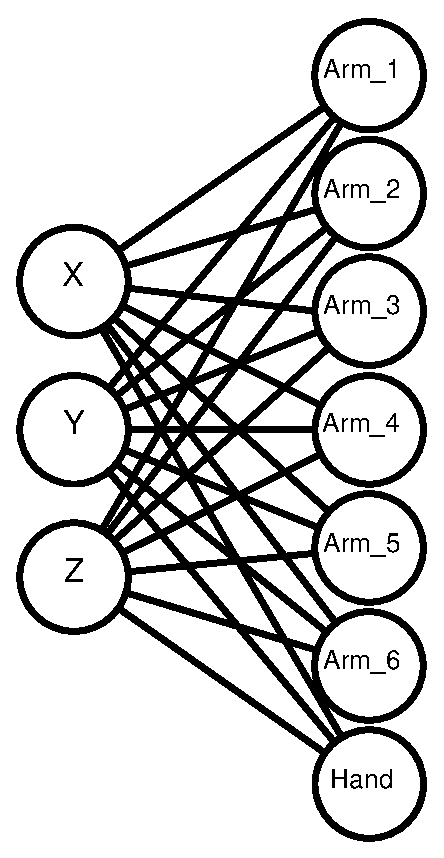
\includegraphics[width=.5\columnwidth]{figures/net.eps}
\caption{Network architecture.}
\label{fig:network}
\end{figure}

\subsubsection{Mutation Strategies}
Three different mutation strategies were implemented to generate new descendants.
The first method uses only one parent and adds or subtracts small random values from its weights.
The other two methods use two parents.
One was a single-point crossover at a random position meaning you take the first n weights from one parent and the remaining ones from the second one.
The last method is a k-point crossover.
At each position this method chooses randomly one of the parents weights.

\subsection{Simplified Problem}
As our first learned approach wasn't really successful we try to reduce the search space for the evolutionary algorithm.
To achieve this we restrict which joints the robot could use to execute the throw.
We fix all rotational joints by setting the respective weights in the neural network to zero because this probably won't impact the robots ability to make a good throw very much.
This reduces the number of weights to be learned from 21 to 12.